\chapter{Theoretical introduction}

\section{Mathematical notation}\label{sec:terminology}
It will be most appropriate to begin by introducing the basic notation that will be used throughout this thesis. This will ensure that any confusion will be avoided, even though the notation is quite standard. 

Notation for random variables using upper case letters of the Latin alphabet is widely used. Typically, the letters used are from the end of the alphabet, i.e. $X,Y$ or $Z$. The realization of a random variable, also known as an observed value or simply an observation, will be denoted by the appropriate lower case letters. Thus, the realization  $x \in \R$ corresponds to the random variable $X$, which holds by analogy for other random variables. However, significant simplification can be achieved if one uses the same notation for random variables and realizations.  

Bold symbols, for instance, $\boldsymbol{x}\in \R^D$ or $\boldsymbol{y} \in \R^D$, will be used to distinguish vectors and scalars. All vectors are assumed to be column vectors, so $\boldsymbol{x} = \left(x_1,x_2,\dots,x_D\right)^\top$ and hence $\boldsymbol{x}^\top$ is a row vector. 

Any matrices will be denoted by blackboard bold Latin letters, for example, if one has $N$ values of $D$-dimensional vector of observations $\boldsymbol{x}_1,\boldsymbol{x}_2,\dots,\boldsymbol{x}_N$, it can be simply combined into a $D \times N$ data matrix $\mathbb{X}$ in which the $j^{\mathrm{th}}$ row of $\mathbb{X}$ corresponds to the row vector $\boldsymbol{x}_j^\top$. The symbol $\mathbb{I}_N$ denotes the square $N \times N$ identity matrix, i.e., matrix with ones on the main diagonal and zeros elsewhere. The set of observations will be denoted by bold uppercase letter, for example $\boldsymbol{X} = \left\lbrace \bx_1,\bx_2,\dots,\bx_N \right\rbrace $.



\section{Probability theory}
Mathematical models are very well described by probability and for this reason, this section will look at some of the basic concepts of probability theory that we will need. The most important such concept is probability density (PDF). The symbol $p(x)$ will be used predominantly for the PDF, which is a function of $x$.  In addition, this will be used for both discrete and continuous $x$. In this way can be achieved significant simplification and unification of all formulas and equations. Any PDF is a non-negative function and its integration over the entire space is equal to 1. This applies to multivariate case as well as it applies to univariate case, therefore integration of joint PDFs $p(\boldsymbol{x}) = p\left(x_1, x_2, \dots, x_D\right)$ over the entire space is also equal to 1. In mathematical terms one can express it as follows
\begin{equation}\label{eq:integrationtoone}
\int_{\R^D}p(\boldsymbol{x})\d{\boldsymbol{x}} = 1.
\end{equation}
In other parts of this thesis we will use conditional PDFs such as $p_{\bt}\left(\bx\right) \equiv p\left(\bx|\bt\right)  $ that are conditioned by known parameters $\bt~\in~\Theta~\subset~\R^s$, where $\Theta$ is called parameter space. The constraint \eqref{eq:integrationtoone} can be always fulfilled by redefining the PDF as
\begin{equation}\label{eq:partitionfunction}
    p_{\bt}\left(\bx\right) = \frac{p_{\bt}^{0}\left(\bx\right)}{Z\left(\bt\right)}, \qquad Z\left(\bt\right) = \int_{\R^D} p_{\bt}^0\left(\bx\right)\d{\bx}, 
\end{equation}
where $p_{\bt}^{0}\left(\bx\right)$ specifies the functional form of the $p_{\bt}\left(\bx\right)$ and does not need to integrate to 1. The normalization constant $Z\left(\bt\right)$ is often called the partition function.

The average value of some function $g(x)$ under a probability distribution $p(x)$ is typically denoted by $\EE{g\left(x\right)}$ and it is called expected value or mean \cite{bishop}. For a continuous variable, expected value are expressed in terms of an integration with respect to the corresponding probability density
\begin{equation}
	\EE{g\left(x\right)} = \int_\R p(x)g(x)\d{x}.
\end{equation} 
In the case of a discrete variable, one has to keep in mind that an integration turns into a sum over all $x$. To specify over which PDF the expectation is calculated, the notation $\mathbb{E}_{p(x)}\left[g\left(x\right)\right]$ can be used.

\section{Supervised Learning}
Supervised learning (SL), in less academic terms called "learning with a teacher", is one of the machine learning tasks  \cite{supervised}.  The goal of this approach is to make a good prediction of the output $y$ (sometimes also called target variable), denoted by the symbol $\hat{y}$, with given input $\boldsymbol{x}$. This prediction is obtained through learning a model $f_{\boldsymbol{\theta}}\left(\boldsymbol{x}\right)\equiv f\left(\boldsymbol{x}; \boldsymbol{\theta}\right)$ that minimizes a loss function  $\pazocal{L}(f_{\boldsymbol{\theta}}(\boldsymbol{x}), y)$ (also known as the error function), where $\boldsymbol{\theta}\in \Theta$ are the parameters of the model. 

To construct this prediction one needs data, hence it is supposed that we have available set of independent and identically distributed (i.i.d.) observations, input--output paired samples denoted by $\pazocal{D} = \left\lbrace \left(x_i , y_i \right)\right\rbrace_{i=1}^N$, eventually, this may in fact be 
\begin{equation}\label{superviseddata}
\pazocal{D} = \left\lbrace\left( \boldsymbol{x}_i , y_i \right)\right\rbrace_{i=1}^N,\quad \boldsymbol{x}_i \in \R^D,\quad y_i \in \R,\quad\forall i = 1,\dots,N.
\end{equation}
The index $i$ will be omitted whenever it is clear
that we are referring to terms associated with a single data point. Such setting is usually known as training data and its applications are regression problems. As an example, we can mention a couple of typically used loss functions for such problems. They are squared error and absolute error
\begin{equation}
\pazocal{L}\left(\widehat{y}, y \right) =
 \begin{cases}
	 \left(y - \widehat{y}\right)^2 \\
	 \abs{y - \widehat{y}} \\
\end{cases}   
\end{equation}
where $\widehat{y} = \widehat{f}_{\boldsymbol{\theta}}\left(\boldsymbol{x}\right) = f(\boldsymbol{x}; \widehat{\boldsymbol{\theta}})$. As we are not quite interested in regression problems in this thesis, we will mainly deal with the second approach. That is classification problems, i.e. when $y \in \pazocal{C}$ is qualitative output and where $\pazocal{C}$ is a finite set.  A typical example is binary classification, where $\pazocal{C} = \left\lbrace0,1 \right\rbrace$. However, classification will be object of interest later in Section \ref{discriminative_modelinmg}.

Here it is clear why the term "learning with a teacher" is used. This metaphor means that the student presents output $\widehat{y}$  and the teacher provides either a correct answer and/or an error that corresponds to the student's answer. 

\subsection{Prediction}
The generalization performance, i.e. the performance on out--of--sample data of the models learned by the algorithm relates to its prediction capability on independent test data $\pazocal{T}$. Assessment of this performance is essentially important in practice, since it conducts the choice of learning
method or model, and gives a measure of the quality of the hereafter
chosen model. There are in fact two seperate goals to achieve:
\begin{enumerate}
    \item \emph{Model selection} - estimating the performance of different models in order to choose the best one.
    \item \emph{Model assessment} - having chosen a final model, estimating its prediction error (generalization error) on new data.
\end{enumerate}
\subsubsection{Cross-Validation}
The simplest and most widely used method for estimating prediction error of the model $\hat{f}_{\boldsymbol{\theta}}$ is called \emph{cross-validation} (CV) \cite{statistics}. It is used for direct estimating of the expected extra-sample error
\begin{equation}
\mathrm{err} = \E\left[\pazocal{L}\left(y, \widehat{y}\right)\right],
\end{equation}
the measure how accurately is the model able to predict output values for previously unseen data - independent test sample. In an ideal case, if sufficient number of data is available, a test set can be set aside and used
to assess the performance of the employed prediction model. Since data are often
scarce, this is usually not possible.

Very elegant solution to this problem is via \emph{K-fold cross-validation} \cite{statistics}. It
uses part of the available data for fitting the model, and a different
part for testing. We split the data into $K$ roughly equal-sized parts, for
example, when $K = 5$, the scenario is shown in Figure \ref{fig:KFOLD}. 
\begin{figure}[h]
\begin{center}
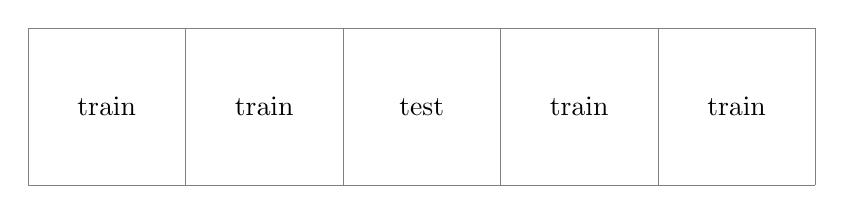
\begin{tikzpicture}
\draw[step=2cm,gray,very thin] (0,0) grid (10,2); 
\draw (5,1) node{test};
\draw (1,1) node{train};
\draw (3,1) node{train};
\draw (7,1) node{train};
\draw (9,1) node{train};
\end{tikzpicture}
\end{center}
\caption{Splitting the data into $K=5$ roughly equal-sized parts.}
\label{fig:KFOLD}
\end{figure}
For the $j^{\mathrm{th}}$ part (third in Figure \ref{fig:KFOLD}), we train the model to the other $K-1$ parts
of the data, and calculate the prediction error of the fitted model when
predicting the $j^{\mathrm{th}}$ part of the data. We repeat this process for $j \in \left\lbrace 1,2,\dots,K\right\rbrace$ and
combine the $K$ estimates of prediction error. Let $\gamma~:~\left\lbrace 1,\dots,N\right\rbrace\rightarrow  \left\lbrace 1,\dots,K\right\rbrace$ be an indexing
function that indicates the partition to which observation $j$ is allocated by
the randomization. Symbol $\hat{f}_{\boldsymbol{\theta}}^{-j}\left(\boldsymbol{x}\right)$ denotes the fitted model, computed with
the $j^{\mathrm{th}}$ part of the data removed. Then the cross-validation estimate of prediction error is defined by
\begin{equation}
\mathrm{CV}\left(\hat{f}_{\boldsymbol{\theta}}\right) = \frac{1}{N}\sum_{i = 1}^{N}\pazocal{L}\left(y_i , \hat{f}_{\boldsymbol{\theta}}^{-\gamma\left(i\right)}\left(\boldsymbol{x}_i\right)\right).
\end{equation}
Typical choices of $K$ are 5 or 10 and even case $K = N$ that is known as \emph{leave-one-out} CV. Generally, there is not an universal way of choosing $K$, since it strongly depends on the available number of data. 
The biggest problem of this method is a fact that it is computionally very expensive, because we usually train many models with different complexity and assess their performance. Let us now analyze the problem of the model complexity. Consider a polynomial regression problem,  where the model is defined by
\begin{equation}
	f_{\boldsymbol{\theta}}(x) = \sum_{i=0}^{s-1}\theta_ix^i.
\end{equation}
 Here, over--fitting occurs very frequently. The complexity of the model of this case is very intuitive, as it is just the order of the polynomial, $s-1$.  Smaller orders of the polynomial (may) give rather poor fits to the data in contrast to a much higher order polynomial giving an excellent fit. However, such a polynomial passes exactly through each data point, oscillates wildly, and gives a poor prediction for the new input variable $x_{0}\in \R$. 
 
To obtain some quantitative insight into the dependence of the generalization performance on model complexity, consider a separate test set of data (testing data) used to assess the performance of the model. 
In general, the prediction error evaluated on the training data for increasing the complexity of the model approaches zero. On the other hand, the prediction error evaluated on the testing data for increasing model complexity is (from a certain point) increasing as well. The typical scenario is illustrated in Figure \ref{fig:Prediction_error}. The goal is then to choose a model that performs best on testing data.
 \begin{figure}[h]
	\centering
	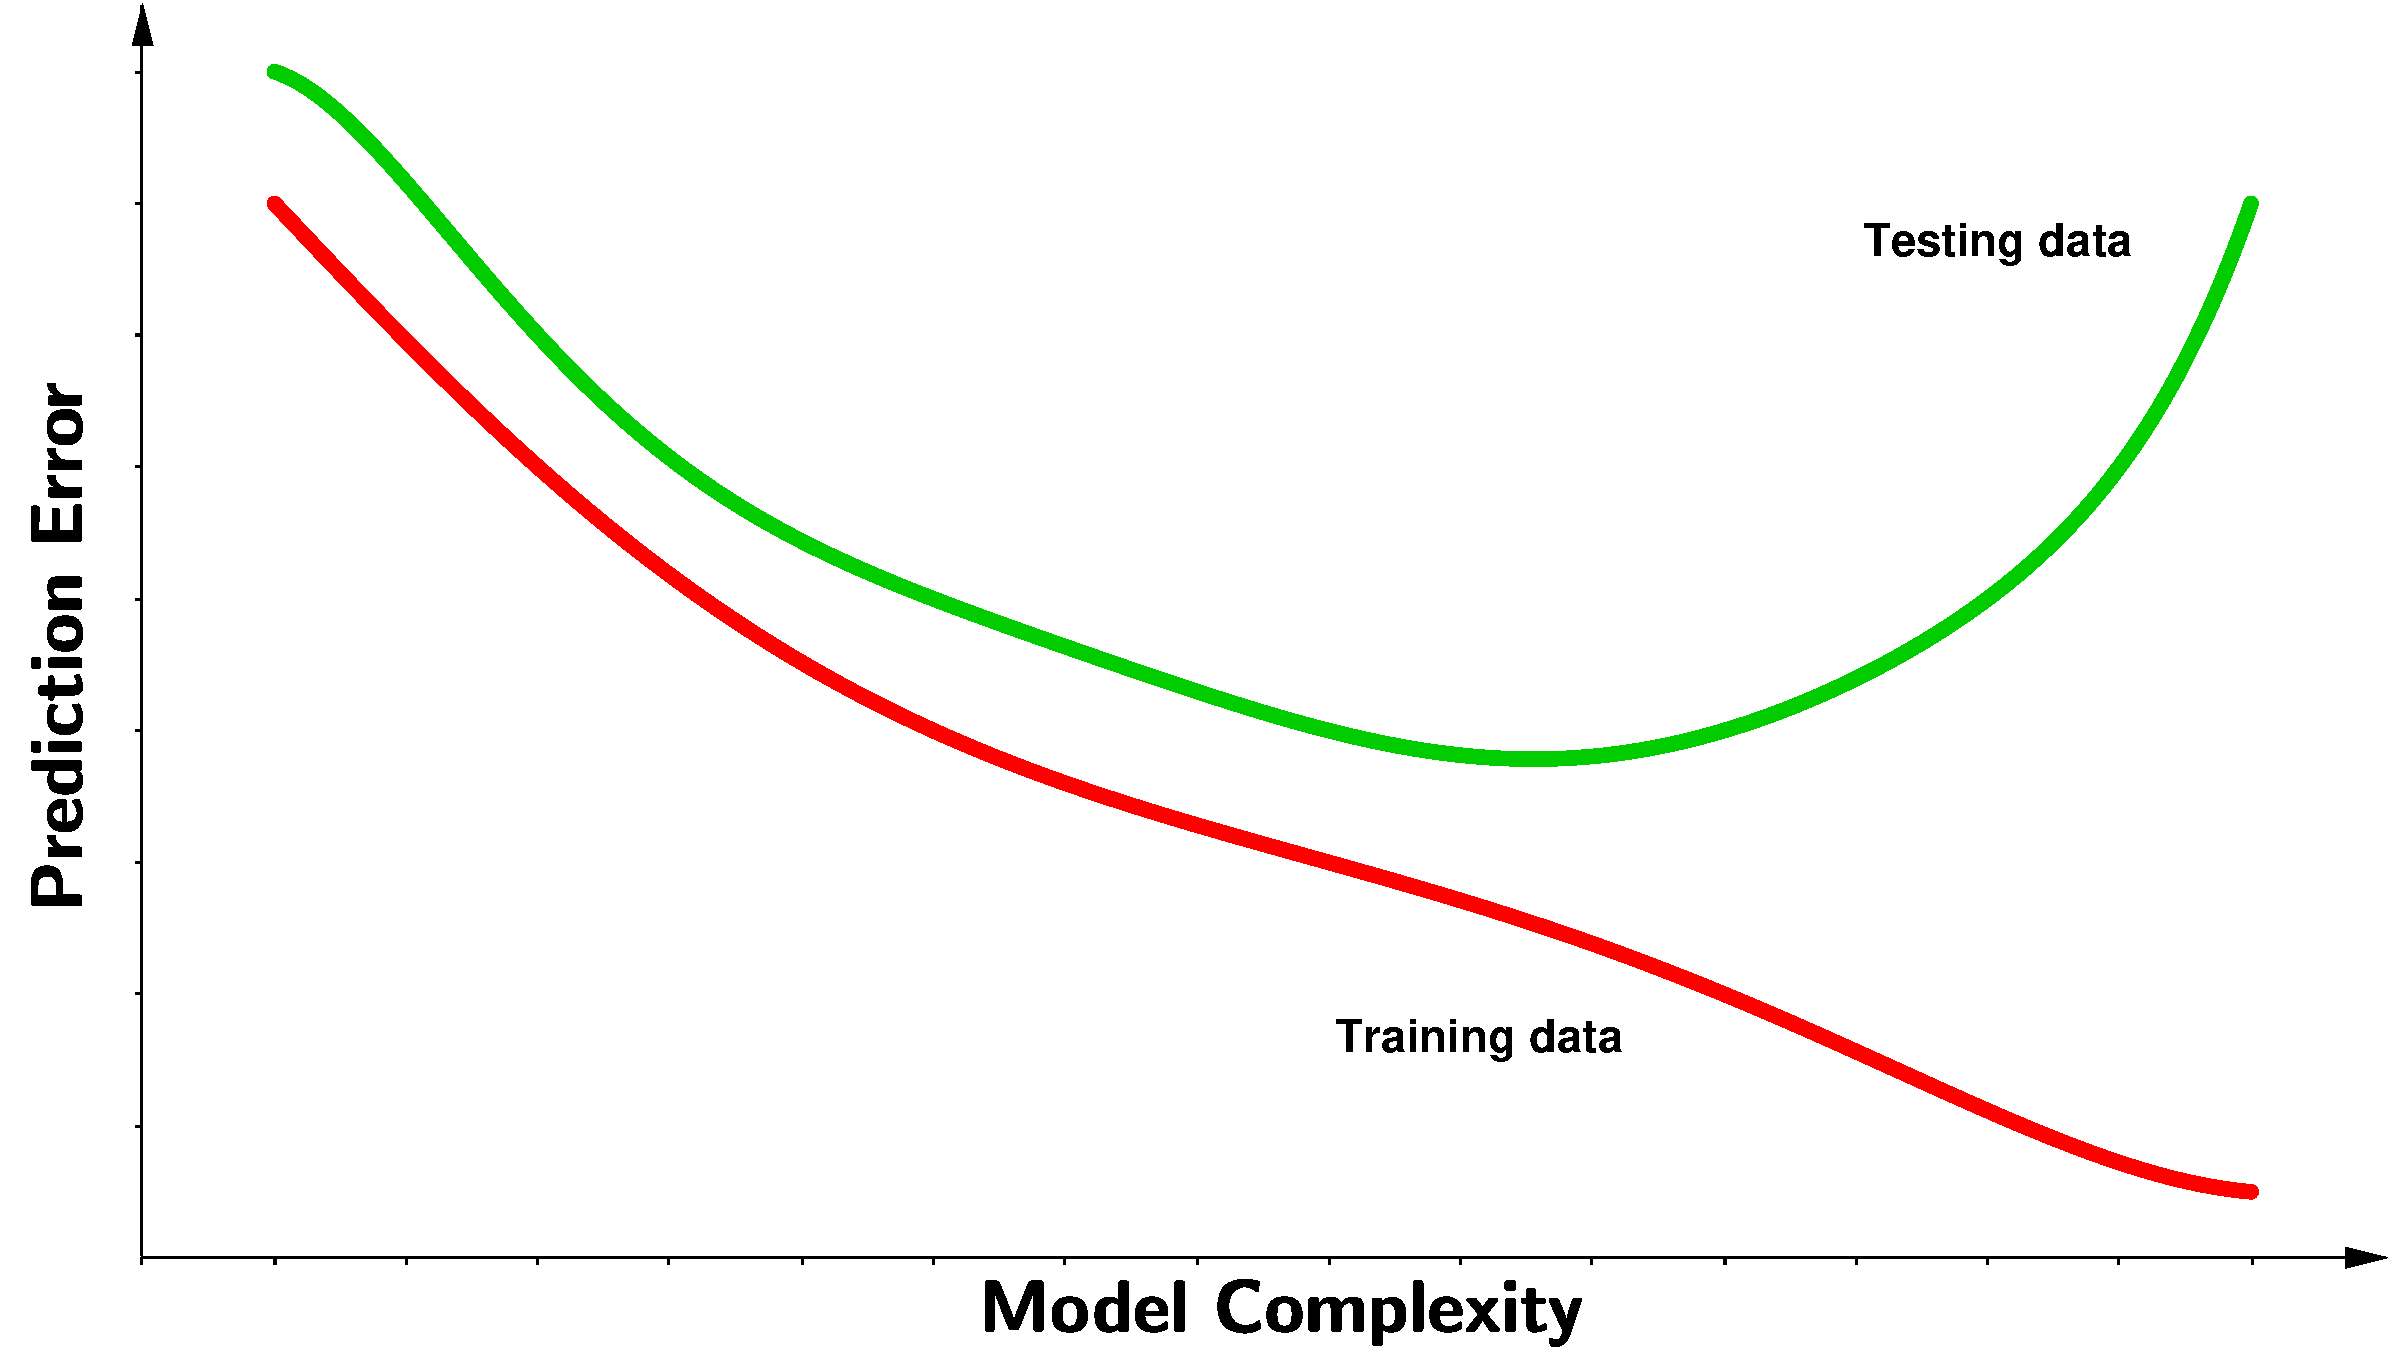
\includegraphics[width=16.0cm]{plots/Images/PE3.pdf}
	\caption{Evaluation of prediction error as a function of model complexity.}%
	\label{fig:Prediction_error}%
\end{figure}
For extremely complicated and complex models that are trained for hours or days, is cross--validation inconvenient approach of estimating the prediction error as we need to train numerous models of this complexity.
\section{Unsupervised learning}
The previous section dealt with input--output paired samples $D$. The second approach is a logical modification of SL, based on data without labels. Such setting is called unsupervised learning (UL) or "learning without a teacher". Unlike SL, one has a set of $N$ observations in the form of $\boldsymbol{X} = \left\lbrace \bx_1^{}, \bx_2,\dots, \bx_N\right\rbrace$ and nothing more. In this case, the student learns without any feedback from a supervisor or teacher providing correct answers. The goal is to directly infer the properties of $p\left( \bx \right)$.




\section{Bayesian Inference}
The Bayesian methodology is a well established approach to statistical inference and became very important technique in statistics and data analysis. As its name suggests, Bayesian statistics is based on application of Bayes' rule. In this chapter, we briefly review basic concept of this approach, which was suggested here \cite{smidl}. 

 Let the measured data be denoted by $\pazocal{D}$, defined according to previous Section \ref{sec:terminology}. A parametric probabilistic model of the data $\pazocal{D}$ is given by the probability density function  $p\left(\pazocal{D}|\boldsymbol{\theta}\right)$, where again $\boldsymbol{\theta}~\in~\Theta$ denotes parameters of the model. The main idea behind Bayesian theory is the treatment of the unknown parameters $\boldsymbol{\theta}$ as a random variable.  Bayes' rule is applied to infer model parameters $\boldsymbol{\theta}$, therefore
 \begin{equation}\label{Bayesinference}
 	p(\boldsymbol{\theta} | \pazocal{D}) = \frac{p(\boldsymbol{\theta}, \pazocal{D})}{p(\pazocal{D})} = \frac{p(\pazocal{D}| \boldsymbol{\theta})p(\boldsymbol{\theta})}{\int_{\Theta}p(\pazocal{D}|\boldsymbol{\theta})p(\boldsymbol{\theta})\d\boldsymbol{\theta}}.
 \end{equation} 
Since $p(\pazocal{D})$ is just the normalization constant, Equation \eqref{Bayesinference} is often simplified to
\begin{equation}
	p(\boldsymbol{\theta} | \pazocal{D}) \propto p(\pazocal{D}| \boldsymbol{\theta})p(\boldsymbol{\theta}).
\end{equation} 
Symbol $\propto$ means equal up to the normalization constant. The term $p(\boldsymbol{\theta} | \pazocal{D})$ is known as the \emph{posterior} distribution, $p(\pazocal{D}| \boldsymbol{\theta})$  as the \emph{observation model}, and $p(\boldsymbol{\theta})$ is called the \emph{prior} distribution of the $\boldsymbol{\theta}$. Note that evaluation of the normalization constant can be computionally expensive, in higher dimension even intractable. 

There is of course many possible options how to obtain $\widehat{\bt}$ from posterior. Popular choices for an optimal value of the point estimate are:
\begin{enumerate}
	\item Maximum A posteriori estimate (MAP)
	\begin{equation}
		\widehat{\boldsymbol{\theta}}_{\mathrm{MAP}} = \argmax_{\boldsymbol{\theta}} p(\boldsymbol{\theta} | \pazocal{D})
	\end{equation}
This method estimates $\boldsymbol{\theta}$ as the mode of the posterior distribution. It appears to be computionally attractive, as it is not necessary to evaluate the normalization constant. 
\item Mean or expected value
\begin{equation}
	\widehat{\boldsymbol{\theta}}_{\mathrm{B}} = \int_{\Theta} \boldsymbol{\theta}~ p(\boldsymbol{\theta} | D) \d\boldsymbol{\theta} = \E_{p(\boldsymbol{\theta} | D) }\left[\boldsymbol{\theta} \right]
\end{equation}
Mean value, unlike MAP estimate, may be very expensive to compute because of the required integration. This may lead to further approximations such as EM algorithm \cite{EM}.
\end{enumerate}	

\subsection{Choice of prior distribution}
For the posterior computation, it is necessary to specify the prior distribution $p(\boldsymbol{\theta})$, unfortunately, this might not be easily determined. This can be achieved through knowledge of previous models, expert knowledge, their combination, or even uncertainty about $\boldsymbol{\theta}$ being a viable option. 

There are also many practical aspects of priors:
\begin{itemize}
	\item \emph{Regularization} - supplementing the data if there are scarce, insufficient data, or poorly defined model. 
	\item \emph{Restrictive conditions} - imposing various restrictions on the parameters $\boldsymbol{\theta}$ reflecting physical constraints. The choice of a prior distribution with bounded support will also result in a posterior distribution with bounded support. 
	\item \emph{Non--informative prior} - if the data are informative enough to make a prediction, it is proposed to choose a prior with minimal impact on the posterior distribution, such as uniform distribution. However, typical choices of non--informative priors are the so--called \emph{Jeffreys priors} \cite{jeffrey}.
\end{itemize}



\subsection{Prediction}
We are not usually interested in the value of $\widehat{\boldsymbol{\theta}}$ itself, but rather, once the model is estimated, we are interested in making a prediction of the output variable $y_0$ for the new input variable $\boldsymbol{x}_0$. Note that the symbol $\pazocal{D}$ contains all previously given data $\boldsymbol{x}$ and $y$. The posterior predictive distribution is then determined by the distribution of $y_0$, marginalized over the posterior
\begin{equation}
	p(y_0 | \boldsymbol{x}_0, \pazocal{D}) =   \int_{\Theta} p(y_0|\boldsymbol{x}_0, \boldsymbol{\theta}) p(\boldsymbol{\theta}|\pazocal{D}) \d\boldsymbol{\theta}.\label{eq:posteriotprediction}
\end{equation} 
When the distribution $p(\boldsymbol{\theta}|\pazocal{D})$ is not available, we have to approximate leveraging the Dirac delta function $\delta(x)$ for which the property
\begin{align}
    \int_{\R} g\left(x\right)\delta(x-x_0)\d{x} = g(x_0)
\end{align}
holds. Once this property is applied to Equation \eqref{eq:posteriotprediction} we get

\begin{equation}
p(y_0 | \boldsymbol{x}_0, \pazocal{D}) = \int_{\Theta} 	p(y_0|\boldsymbol{x}_0, \boldsymbol{\theta}) \delta(\boldsymbol{\theta} - \widehat{\boldsymbol{\theta}})\d\boldsymbol{\theta} = p(y_0|\boldsymbol{x}_0, \widehat{\boldsymbol{\theta}}),
\end{equation}
causing an error. In typical MAP, this is known as \emph{over--fitting}. 

 
